\documentclass[11pt, a4paper, twoside]{article}   	% use "amsart" instead of "article" for AMSLaTeX format

\usepackage{geometry}                		% See geometry.pdf to learn the layout options. There are lots.
\usepackage{pdfpages}
\usepackage{caption}
\usepackage{minted}
\usepackage[german]{babel}			% this end the next are needed for german umlaute
\usepackage[utf8]{inputenc}
\usepackage{color}
\usepackage{graphicx}
\usepackage{titlesec}
\usepackage{fancyhdr}
\usepackage{lastpage}
\usepackage{hyperref}
\usepackage[autostyle=false, style=english]{csquotes}
\usepackage{mathtools}
\usepackage{tabularx}
% http://www.artofproblemsolving.com/wiki/index.php/LaTeX:Symbols#Operators
% =============================================
% Layout & Colors
% =============================================
\geometry{
   a4paper,
   total={210mm,297mm},
   left=20mm,
   right=20mm,
   top=20mm,
   bottom=30mm
 }	

\definecolor{myred}{rgb}{0.8,0,0}
\definecolor{mygreen}{rgb}{0,0.6,0}
\definecolor{mygray}{rgb}{0.5,0.5,0.5}
\definecolor{mymauve}{rgb}{0.58,0,0.82}

\setcounter{secnumdepth}{4}


% the default java directory structure and the main packages
\newcommand{\srcDir}{../src/}
\newcommand{\imageDir}{./images/}
% =============================================
% Code Settings
% =============================================
\newenvironment{code}{\captionsetup{type=listing}}{}
\newmintedfile[mSourceFile]{matlab}{
	linenos=true, 
	frame=single, 
	breaklines=true, 
	tabsize=2,
	numbersep=5pt,
	xleftmargin=10pt,
	baselinestretch=1,
	fontsize=\footnotesize
}
\newmintinline[mInlineSource]{matlab}{}
\newminted[mSource]{matlab}{
	breaklines=true, 
	tabsize=2,
	autogobble=true,
	breakautoindent=false
}
% =============================================
% Page Style, Footers & Headers, Title
% =============================================
\title{Übung 1}
\author{Thomas Herzog}

\lhead{Übung 1}
\chead{}
\rhead{\includegraphics[scale=0.10]{FHO_Logo_Students.jpg}}

\lfoot{S1610454013}
\cfoot{}
\rfoot{ \thepage / \pageref{LastPage} }
\renewcommand{\footrulewidth}{0.4pt}
% =============================================
% D O C U M E N T     C O N T E N T
% =============================================
% =============================================
% 2016.10.13: 1 
% 2016.10.14: 2
% =============================================

\pagestyle{fancy}
\begin{document}
\setlength{\headheight}{15mm}
\includepdf[pages={1,2}]{Uebungszettel02.pdf}

% Section gramar and basics 
\section{Kontinuierliche Modellierung}
\label{sec:continous-modeling}
Dieser Abschnitt beschäftigt sich mit der Aufgabenstellung 1 der zweiten Übung. 

\subsection{Erstes Blockdiagramm für 1a 1}
Dieser Abschnitt beschäftigt ich mit dem Aufstellen der Gleichungen in A, B, C Normalform, die aus den gegebenen Blockdiagramm aus Aufgabenstellung 1a abgeleitet wurden.
\newline
\newline
$U= \begin{bmatrix}
	u_1 \\[0.3em]
	u_2 \\[0.3em]
\end{bmatrix}
,
X = \begin{bmatrix}
	z \\[0.3em]
	v \\[0.3em]
	x \\[0.3em]
\end{bmatrix}
,
Y=\begin{bmatrix}
	y_1 \\[0.3em]
	y_2 \\[0.3em]
	y_3 \\[0.3em]
\end{bmatrix}
\newline
\newline
\newline
z'= 0*z + 0*v + 0*x + 2*u_1 + 2*u_2 \hspace{2mm} \equiv \hspace{2mm} 2*u_1 + 2*u_2
\newline
v'= 1*z + 0*v + 0*x + 0*u_1 - 1*u_2 \hspace{2mm} \equiv \hspace{2mm} z - u_2
\newline
x'= 0*z + 1*v + 0*x + 0*u_1 + 0*u_2 \hspace{2mm} \equiv \hspace{2mm} v 
\newline
\newline
y_1 = 0*z + 0*v + 0* x \hspace{30mm} \equiv \hspace{2mm} 0
\newline
y_2 = 0*z + 1*v + 0* x \hspace{30mm} \equiv \hspace{2mm} v
\newline
y_3 = 0*z + 0*v + 1* x \hspace{30mm} \equiv \hspace{2mm} x
\newline
\newline
\newline
X'=A*X + B * U
\newline
\newline
X'= \begin{bmatrix}
	0 & 0 & 0 \\[0.3em]
	1 & 0 & 0 \\[0.3em]
	0 & 1 & 0 \\[0.3em]
\end{bmatrix}
* 
\begin{bmatrix}
	z \\[0.3em]
	v \\[0.3em]
	x \\[0.3em]
\end{bmatrix}
+
\begin{bmatrix}
	2 & 2\\[0.3em]
	0 & -1 \\[0.3em]
	0 & 0 \\[0.3em]
\end{bmatrix}
*
\begin{bmatrix}
	u_1 \\[0.3em]
	u_2 \\[0.3em]
\end{bmatrix}
\newline
\newline
\newline
\newline
Y=C*X
\newline
\newline
Y=
\begin{bmatrix}
	0 & 0 & 0 \\[0.3em]
	0 & 1 & 0 \\[0.3em]
	0 & 0 & 1 \\[0.3em]
\end{bmatrix}
*
\begin{bmatrix}
	z \\[0.3em]
	v \\[0.3em]
	x \\[0.3em]
\end{bmatrix}
$
\newpage

\subsection{Zweites Blockdiagramm für 1a 2}
Dieser Abschnitt beschäftigt ich mit dem Aufstellen der Gleichungen in A, B, C Normalform, die aus den gegebenen Blockdiagramm aus Aufgabenstellung 1b abgeleitet wurden.
\newline
\newline
$U= \begin{bmatrix}
	u_1 \\[0.3em]
	u_2 \\[0.3em]
	u_3 \\[0.3em]
\end{bmatrix}
,
X = \begin{bmatrix}
	z \\[0.3em]
	x \\[0.3em]
\end{bmatrix}
,
Y = \begin{bmatrix}
	y1 \\[0.3em]
	y2 \\[0.3em]
\end{bmatrix}
\newline
\newline
\newline
z'= 0*z + 0*x + 0*u_1 - 5*u_2 + 0*u_3\hspace{15mm} \equiv \hspace{2mm} - 5*u_2
\newline
x'= 1*z + 1*x + 0*u_1 + (-2*u_2 + 1) + 1*u_3 \hspace{2mm} \equiv \hspace{2mm} z + x + (-2*u_2 + 1) + u_3
\newline
\newline
y_1 = 0*z + 0* x \hspace{57mm} \equiv \hspace{2mm} 0
\newline
y_2 = 0*z + 1* x \hspace{57mm} \equiv \hspace{2mm} x
\newline
\newline
\newline
X'=A*X + B * U
\newline
\newline
X'= \begin{bmatrix}
	0 & 0 \\[0.3em]
	1 & 1 \\[0.3em]
\end{bmatrix}
* 
\begin{bmatrix}
	z \\[0.3em]
	x \\[0.3em]
\end{bmatrix}
+
\begin{bmatrix}
	0 & -5 & 0 \\[0.3em]
	0 & (-2*u_2 + 1) & 1 \\[0.3em]
\end{bmatrix}
*
\begin{bmatrix}
	u_1 \\[0.3em]
	u_2 \\[0.3em]
	u_3 \\[0.3em]
\end{bmatrix}
\newline
\newline
\newline
\newline
Y=C*X
\newline
\newline
Y =
C = \begin{bmatrix}
	0 & 0 \\[0.3em]
	0 & 1 \\[0.3em]
\end{bmatrix}
*
\begin{bmatrix}
	z \\[0.3em]
	x \\[0.3em]
\end{bmatrix}
$
\newpage

\subsection{Erstes System als Blockschaltbild für 1b 1}
Dieser Abschnitt beschäftigt sich mit der Aufgabenstellung 1b 1. Die angeführten Vektoren wurden angenommen.
\newline
$
U= \begin{bmatrix}
	u_1 \\[0.3em]
	u_2 \\[0.3em]
\end{bmatrix}
,
X = \begin{bmatrix}
	x \\[0.3em]
	v \\[0.3em]
	z \\[0.3em]
\end{bmatrix}
$
\begin{figure}[h]
\centering
\includegraphics[scale=0.70,angle=90]{\imageDir/aufgabe_b1.JPG}
\caption{Blockschaltbild zum System aus Aufgabenstellung 1b 1}
\label{fig:exercise-b1}
\end{figure}
\newpage

\subsection{Zweites System als Blockschaltbild für 1b 2}
Dieser Abschnitt beschäftigt sich mit der Aufgabenstellung 1b 2. Die angeführten Vektoren wurden angenommen.
\newline
$
U= \begin{bmatrix}
	u_1 \\[0.3em]
	u_2 \\[0.3em]
\end{bmatrix}
,
X = \begin{bmatrix}
	x \\[0.3em]
	v \\[0.3em]
\end{bmatrix}
\newline
\newline
\newline
$
\begin{figure}[h]
\centering
\includegraphics[scale=0.8,angle=90]{\imageDir/aufgabe_b2.JPG}
\caption{Blockschaltbild zum System aus Aufgabenstellung 1b 2}
\label{fig:exercise-b1}
\end{figure}
\newpage

\subsection{Fehlerhaftes System in A, B, C Normalform für 1c}
Dieser Abschnitt beschäftigt sich mit der Aufgabenstellung 1c. Die für das System aufgestellte $C$-Matrix ist falsch, da dieses System drei Systemzustände besitzt und daher die $C$-Matrix drei Spalten haben muss, nähmlich so viele Spalten wie es Systemzustände gibt.
\newline
\newline
$
Y=C*X \hspace{5mm} wobei \hspace{3mm} 
X= \begin{bmatrix}
	x \\[0.3em]
	v \\[0.3em]
	z \\[0.3em]
\end{bmatrix}
\hspace{3mm} und \hspace{3mm} 
C = \begin{bmatrix}
	1 & 0 & 0 \\[0.3em]
	2 & 0 & 0 \\[0.3em]
	3 & 0 & 0 \\[0.3em]
\end{bmatrix}
$

\subsection{System als Blockschaltbild und in A, B, C Normalform für 1d}
Dieser Abschnitt beschäftigt sich mit der Aufgabenstellung 1d.  
\newline
$
X = \begin{bmatrix}
	a \\[0.3em]
	b \\[0.3em]
	c \\[0.3em]
\end{bmatrix}
,
U = \begin{bmatrix}
	i_1 \\[0.3em]
	i_2 \\[0.3em]
\end{bmatrix}
\newline
\newline
\newline
X'=A*X+B*U
\newline
\newline
X'= \begin{bmatrix}
	2 & 4 & -2 \\[0.3em]
	0 & 4 & -1 \\[0.3em]
	0 & 0 & -1 \\[0.3em]
\end{bmatrix}
*
\begin{bmatrix}
	a \\[0.3em]
	b \\[0.3em]
	c \\[0.3em]
\end{bmatrix}
+
\begin{bmatrix}
	2 & 0 \\[0.3em]
	0 & 1 \\[0.3em]
	3 & 0 \\[0.3em]
\end{bmatrix}
*
\begin{bmatrix}
	i_1 \\[0.3em]
	i_2 \\[0.3em]
\end{bmatrix}
\newline
\newline
\newline
\newline
Y=C*X
\newline
\newline
Y=
\begin{bmatrix}
	3 & 0 & 0 \\[0.3em]
	0 & -1 & 0 \\[0.3em]
	1 & 0 & -1 \\[0.3em]
\end{bmatrix}
*
\begin{bmatrix}
	a \\[0.3em]
	b \\[0.3em]
	c \\[0.3em]
\end{bmatrix}
=
\begin{bmatrix}
	(3*a) \\[0.3em]
	(-b) \\[0.3em]
	(a-c) \\[0.3em]
\end{bmatrix}
$

\begin{figure}
\centering
\includegraphics[scale=0.7,angle=90]{\imageDir/aufgabe_b3.JPG}
\caption{Blockschaltbild zum System aus Aufgabenstellung 1c}
\label{fig:exercise-b1}
\end{figure}
\ \newpage

\section{Kontinuierliche Simulation}
\label{sec:continous-simulation}
Im Gegensatz zu linearen System können bei nicht linearen Systemen die Werte nicht zu jeden Zeitpunkt exakt berechnet werden. Daher wird bei nicht linearen Systemen (kontinuierliche Systeme) die Werteveränderung zum Zeitpunkt $t$ annäherungsweise (numerische Integration) berechnet. Mit der numerischen Integration können alle kontinuierlichen Systeme, die durch Differenzialgleichungen dargestellt werden können, linear oder nicht,  simuliert werden. Es können mit der numerischen Integration die Wertänderung zum Zeitpunkt $t$ nur annäherungsweise berechnet werden, wodurch zwangsweise Fehler gemacht werden. Die Fehler hängen ab von der Schrittweite $h$ und der gewählten Methode der numerischen Integration.
\newline
\newline
Ideal wäre die Schrittweite $h=0$, da dadurch überhaupt keine Fehler gemacht werden würden, es würde aber unendlich viel Laufzeit in Anspruch nehmen und ist daher nicht in endlicher Zeit lösbar. Eine zu große Schrittweite wie z.B. $h=10$ würde zu einen zu großen Fehler führen und ein Teil des Verhaltens des Systems könnte nicht erfasst werden. Auch ist eine über die Simulationsdauer gewählte Schrittweite $h$ vielleicht auch nicht immer passend, wenn es z.B. wenig Veränderungen im System gibt, eine zu kleine Schrittweite unnötig ist und bei starken Veränderungen eine zu kleine Schrittweite zu wenig ist. Daher bitten einige Methoden der numerischen Integration wie z.B. die Methode nach \emph{Runge Kutta} die Möglichkeit der Anpassung der Schrittweite während der Simulation an, wodurch die Simulation effizienter durchlaufen werden kann.
\newline
\newline
Wie schon erwähnt ist es nicht möglich eine Simulation eines nicht linearen Systems zu realisieren, ohne Fehler vollständig zu vermeiden. Es ist nur möglich den Fehler in einem Bereich zu halten, der für die Simulation akzeptabel ist. Die beiden Fehlertypen lokale Fehler und globale Fehler beschreiben den Fehler der entweder pro berechneten Schritt oder über die gesamte Simulationsdauer gemacht wird. Für eine Simulation ist der globale Fehler von größerem Interesse, da die pro Schritt gemachten Fehler bei einem akzeptablen globalen Fehler nicht mehr ins Gewicht fallen.
\newline
\newline
Die folgende Auflistungen zeigen die Methoden der numerischen Integration, die sich in die beiden Gruppen \emph{Einschrittverfahren} und \emph{Mehrschrittverfahren} aufteilen.
\newline
\newline
\textbf{Einschrittmethoden:}
\begin{enumerate}
	\item Euler Integration
	\item Methode von Heun
	\item Runge Kutta
\end{enumerate}
\textbf{Mehrschrittmethoden:}
\begin{enumerate}
	\item Adams Bashford
	\item Adams Moulton
\end{enumerate}
\ \newline
Die beiden Gruppen \emph{Einschritt-} und \emph{Mehrschrittverfahren} unterscheiden sich im Bezug auf die einbezogenen Werte bei der Berechnung, wobei bei Einschrittverfahren immer nur einen Wert verwenden und die Mehrschrittverfahren vergangene und zukünftige Werte miteinbeziehen können. Die Wahl der richtigen Methode für die Simulation hängt ab von der Simulation selbst, der benötigten Fehlertoleranz und dem Laufzeitverhalten. Allgemein wird das Einschrittverfahren nach \emph{Runge Kutta} als angemessen angesehen.
\newpage 

\subsection{Euler Integration}
Mit der Euler Integration $y_{i+1}=y_i+h*f(y_i)$, die ein Einschrittverfahren ist, wird die Wertänderung über ein rechtwinkliges Dreieck ermittelt. Dieses Verfahren ist das schnellste der Verfahren, da pro Schritt nur einmal die Funktion $f(y_i)$ aufgerufen werden muss. Der globale Fehler ($O(h)$) verhält sich linear zur gewählten Schrittweite.
\newline
\newline
Bsp.: $h=10 \rightarrow O(h), h'=h/2 \rightarrow O(h')=O(h/2)=$

\begin{figure}[h]
\centering
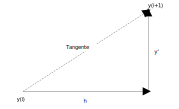
\includegraphics[scale=1]{\imageDir/euler_integration.JPG}
\caption{Dreieck zur Berechnung der Steigung der Wertänderung}
\label{fig:euler-integration}
\end{figure}

\subsection{Methode von Heun}
Mit der Methode von Heun $y_{i+1}=y_i+h/2*(f(y_i) + f(y_i+h*f(y_i)))$, die auch ein Einschrittverfahren ist, wird der nächste Wert im Gegensatz zur Euler Integration über ein Trapez ermittelt. Der globale Fehler ($O(h^2)$) verhält sich quadratisch zur gewählten Schrittbreite $h$. 
\newline
\newline
Bsp.: $h=10 \rightarrow O(h^2), h'=h/2 \rightarrow O(h')=O((h/2)^2)$
\newline
\newline
Der globale Fehler nimmt daher bei geringerer Schrittbreite deutlich mehr ab als bei der Euler Integration.

\begin{figure}[h]
\centering
\includegraphics[scale=1]{\imageDir/method_heun.JPG}
\caption{Trapez zur Berechnung der Steigung der Wertänderung}
\label{fig:euler-integration}
\end{figure}

\subsection{Runge Kutta}
Die Methode von Runge Kutta ist ein vierstufiges Einschrittverfahren, das mit Schrittweitenanpassung arbeitet. Es wird ein \emph{Threshold} des erlaubten Fehlers und die neue Schrittweite für den Fehlerfall definiert, die angewendet wird, wenn der \emph{Threshold}  überschritten wurde. Mit der dynamischen Anpassung der Schrittweite kann bei einer Simulation der Rechenaufwand bei wenig Änderungen vermindert werden. Nehmen die Änderungen zu, wird der Fehler bei der Berechnung größer, wodurch der \emph{Threshold} überschritten wird und die Schrittweite auf den definierten Wert verkleinert wird. Damit wird der Fehler wieder kleiner, was mit einem Rechenaufwand einhergeht.
\newpage

\begin{figure}[h]
\centering
\includegraphics[scale=1]{\imageDir/runge_kutta.JPG}
\caption{\emph{Runge Kutta} Verfahren mit Schrittweitenanpassung}
\label{fig:euler-integration}
\end{figure}

\subsection{Mehrschrittverfahren}
Bei dem Mehrschrittverfahren nach \emph{Adams Bashford} werden nur vergangene Werte bei der Berechnung des nächsten Werts miteinbezogen. Bei dem Mehrschrittverfahren nach \emph{Adams Moulton} werden zusätzlich zu den vergangen Werten auch angenommene Zukunftswerte bei der Berechnung des nächsten Werts miteinbezogen. Bei beiden Verfahren werden empirische Faktoren verwendet, die sich über die Zeit als gute Faktoren bewährt haben. Die Mehrschrittverfahren haben ein besseres Laufzeitverhalten sind aber schwerer zu implementieren.
\end{document}
